\documentclass[xcolor=dvipsnames]{beamer} % dvipsnames gives more built-in colors
\usepackage{graphicx}
\usetheme{Luebeck}
\useoutertheme{infolines} % Alternatively: miniframes, infolines, split
\useinnertheme{circles}
\usepackage{subcaption}
\usepackage{listings}
\usepackage{tikz,tikz-3dplot}
\usetikzlibrary{calc,arrows}
\usepackage{xcolor}
\lstset{
	basicstyle=\ttfamily\tiny,
	basewidth=0.65em,
	commentstyle=\ttfamily,
	tabsize=2,
	keywordstyle=\bfseries\sffamily,
	showstringspaces=false,
	numberstyle=\tiny,
	numbersep=2.5pt,
	keywordstyle=\bfseries\ttfamily,
	breaklines=true
}
\lstnewenvironment{pseudoc}{\lstset{frame=lines,mathescape=true, language = C++, basicstyle=\ttfamily\small, basewidth=0.55em}}{}

\definecolor{UBCblue}{rgb}{0.04706, 0.13725, 0.26667} % UBC Blue (primary)

\usecolortheme[named=MidnightBlue]{structure}
%\usecolortheme[named=Mahogany]{structure} % Sample dvipsnames color

\title[Valutazione del Contatto Pneumatico/Strada]{Valutazione Real-Time del Contatto Pneumatico/Strada con Algoritmi Dedicati}
\date{}

\usepackage{fontspec}
\defaultfontfeatures{Mapping=tex-text}
\setromanfont[Ligatures={Common}]{Adobe Caslon Pro}
\usefonttheme{serif}

\begin{document}

\begin{frame}
	\vspace{-.5cm}
	\titlepage
	\vspace{-3cm}
	\begin{center}
		\begin{tabular}{cc}
			\begin{minipage}[t]{0.45\textwidth}
				Relatore:\\
				\textbf{Prof. Enrico Bertolazzi}\\
				Università di Trento\\[.3cm]
				Co-relatore:\\
				\textbf{Dott. Ing. Matteo Ragni}\\
				AnteMotion S.r.l
			\end{minipage}
			& 
			\begin{minipage}[t]{0.45\textwidth}
				\begin{flushright}
					Candidato:\\
					\textbf{Davide Stocco}
				\end{flushright}
			\end{minipage}
		\end{tabular}
	\end{center}
	\begin{figure}
		\flushright
		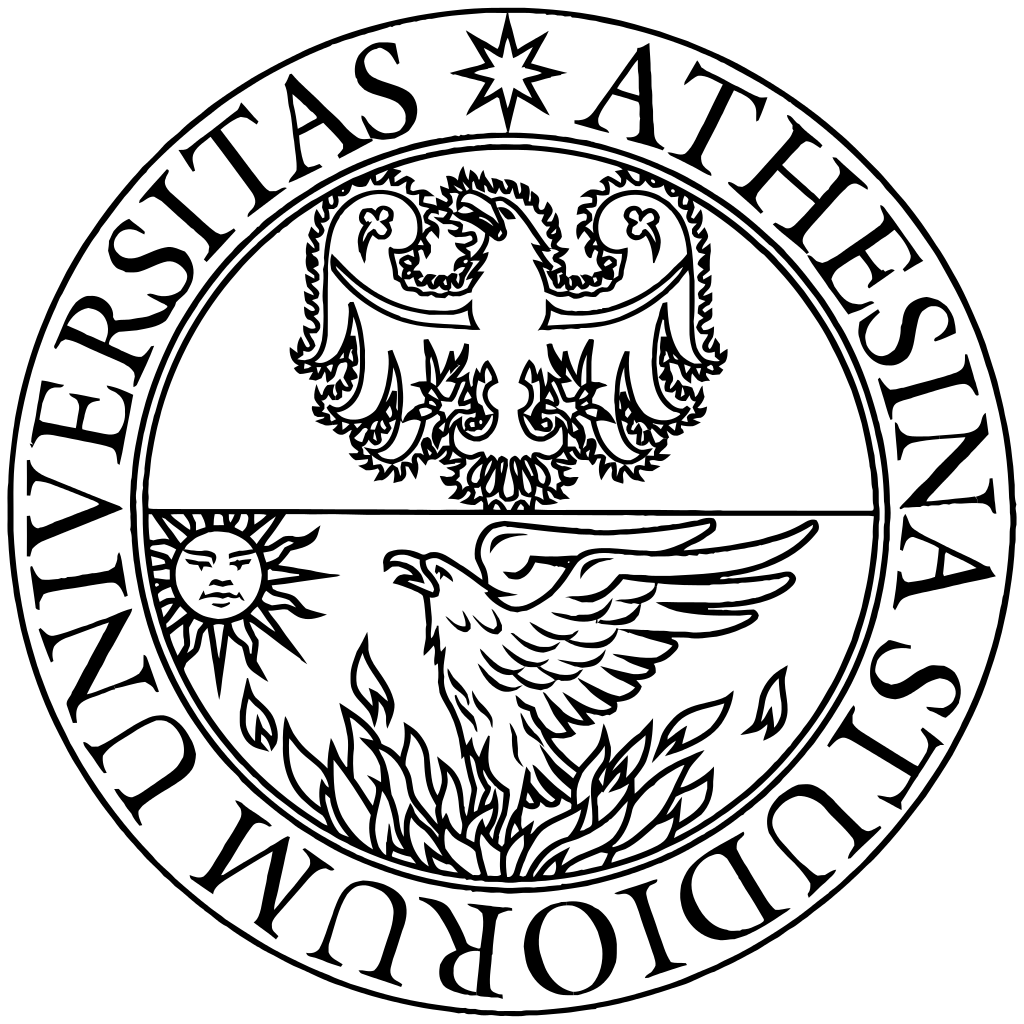
\includegraphics[width=0.1\linewidth]{../Figures/unitn}
		\quad
		
\includegraphics[width=0.42\linewidth]{../Figures/ante}
	\end{figure}
\end{frame}

\author{Davide Stocco}
	
\begin{frame}
	\Large{Obiettivi della Tesi}:
	\normalsize
	\begin{enumerate}
		\item Simulatore\textit{ Software in the Loop} (SIL) e \textit{Hardware in	the Loop} (HIL)
		\item Applicazione in tempo reale
		\item Sviluppo di una libreria \texttt{C++}
	\end{enumerate}
	\\[1cm]
	\Large {Intersezione con pneumatico/strada}:
	\normalsize
	\begin{enumerate}
		\item Analisi sintattico-grammaticale del formato \texttt{rdf}
		\item Modellazione geometrica dello pneumatico
		\item Implementazione degli algoritmi per intersecare entità geometriche:
		\item Valutazione del contatto mediante modelli di contatto
	\end{enumerate}
\end{frame}

\begin{frame}[fragile]
	\Large {Il formato \texttt{rdf}} per le superfici stradali:
	\normalsize
	\begin{figure}
		\centering
		\begin{subfigure}{.5\linewidth}
\begin{pseudoc}
[NODES]
{ id x_coord y_coord z_coord }
0 2.64637 35.8522 -1.59419e-005 
1 4.54089 33.7705 -1.60766e-005 
2 4.52126 35.8761 -1.62482e-005 
3 2.66601 33.7456 -1.57714e-005 
4 0.771484 35.8282 -1.56367e-005 
... ... ... ...
[ELEMENTS]
{ n1 n2 n3 mu }
1 2 3 1.0 
2 1 4 1.0 
... ... ... ...
\end{pseudoc}
		\end{subfigure}
	\end{figure}
%Altri parametri non considerati: \texttt{X\_SCALE}, \texttt{Z\_SCALE}, \texttt{Z\_SCALE}, \texttt{ORIGIN}, \texttt{ORIGIN} e \texttt{ORIENTATION}.
\end{frame}

\begin{frame}[fragile]
	\Large{Analisi sintattico-grammaticale del formato \texttt{rdf}}:
	\normalsize
	\begin{enumerate}
		\item Estrazione dei \texttt{[NODES]}
		\item Estrazione degli \texttt{[ELEMENTS]}
		\item Istanziamento dei triangoli componenti la \textit{mesh}
		\item[$\textcolor{red}{\textbf{!!!}}$] \textcolor{red}{\textbf{ Non esiste uno \textit{standard} per questo formato}}
	\end{enumerate}
\begin{figure}
	\centering
	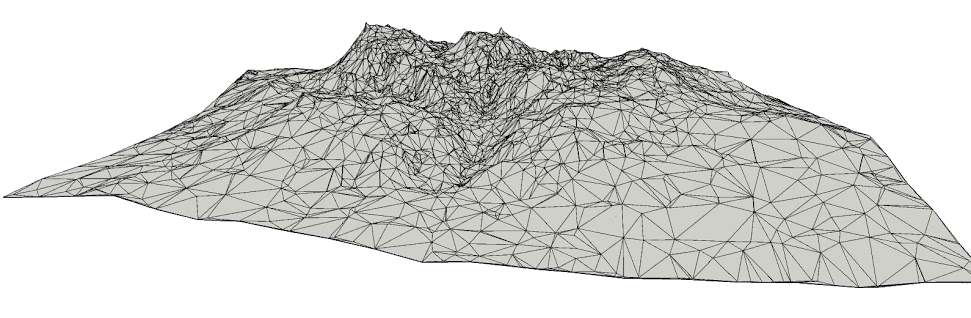
\includegraphics[width=0.7\linewidth]{../Figures/mesh}
\end{figure}
\vspace{-0.3cm}
\begin{pseudoc}
TireGround::RDF::MeshSurface Road(
"./file.rdf" // Path to the *.rdf file
);
\end{pseudoc}
\end{frame}

\begin{frame}
	\Large{Albero delle \textit{Axis-Aligned Bounding Boxes} (AABB)}:
	\normalsize
	\begin{enumerate}
		\item Raggruppamento ricorsivo delle AABB dei triangoli della \textit{mesh}
		\item Diminuzione in scala logaritmica del numero di comparazioni
		\item Solo confronti logici
	\end{enumerate}
	\begin{figure}
		\centering
		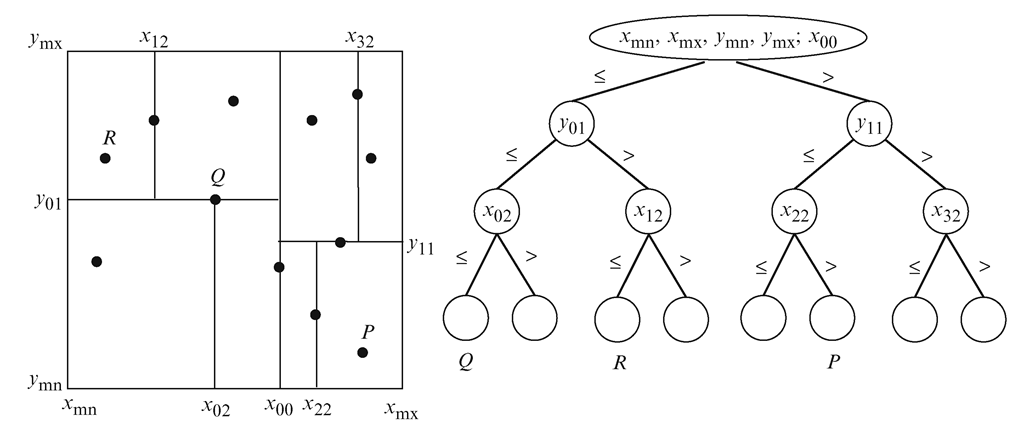
\includegraphics[width=0.85\linewidth]{../Figures/AABB}
	\end{figure}
\end{frame}

\begin{frame}
	\Large {Descrizione geometrica dello pneumatico secondo \textit{European Tire and Rim Technical Organization} (ETRTO)}:
	\begin{figure}
		\centering
		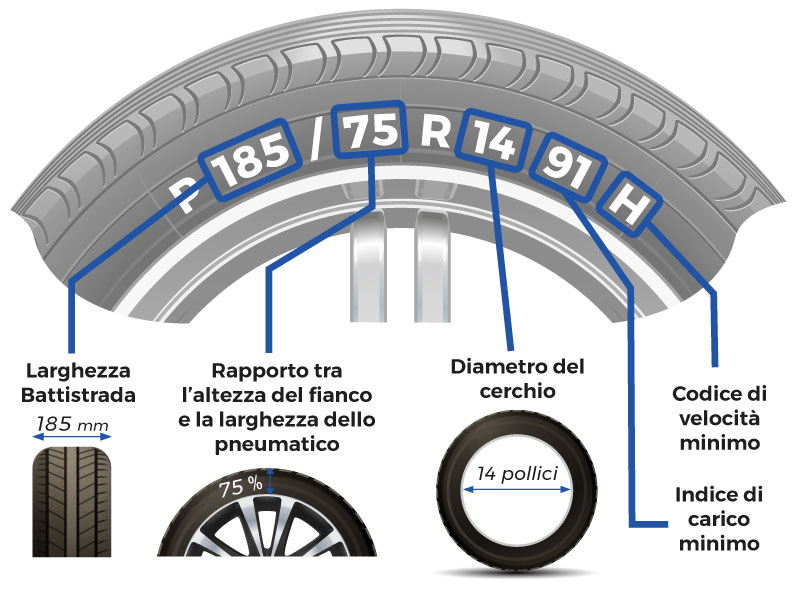
\includegraphics[width=0.7\linewidth]{../Figures/tire_measures}
	\end{figure}
\end{frame}

\begin{frame}
	\Large {Rappresentazione tramite uno o più dischi indeformabili}:
	\begin{figure}
		\hfill
		\begin{subfigure}{0.45\linewidth}
			\centering
			\tdplotsetmaincoords{70}{110}
			\tdplotsetrotatedcoords{90}{90}{0}
			\begin{tikzpicture}[tdplot_main_coords,scale=0.65]	
			\draw[-stealth] (0,0,0) -- (8,0,0) node[anchor=north east]{$x_C$};
			\draw[-stealth] (0,0,0) -- (0,3,0) node[anchor=west]{$y_C$};
			\draw[-stealth] (0,0,0) -- (0,0,5) node[anchor=west]{$z_C$};
			\def\r{4};
			
			\begin{scope}[tdplot_rotated_coords]
			\tdplotdrawarc[tdplot_rotated_coords,thick]{(0,0,0)}{\r}{0}{360}{}{}
			\end{scope}
			\end{tikzpicture}
			\small{Disco singolo}
		\end{subfigure}
		\hfill
		\begin{subfigure}{0.45\linewidth}
			\centering
			\tdplotsetmaincoords{70}{110}
			\tdplotsetrotatedcoords{90}{90}{0}
			\begin{tikzpicture}[tdplot_main_coords,scale=0.65]
				\draw[-stealth] (0,0,0) -- (9,0,0) node[anchor=north east]{$x_C$};
				\draw[-stealth] (0,0,0) -- (0,3.5,0) node[anchor=west]{$y_C$};
				\draw[-stealth] (0,0,0) -- (0,0,5) node[anchor=west]{$z_C$};
				\def\r{4};
				
				\begin{scope}[tdplot_rotated_coords]
				\tdplotdrawarc[tdplot_rotated_coords,thick]{(0,0,1.6)}{\r-0.5}{0}{360}{}{}
				
				\tdplotdrawarc[tdplot_rotated_coords,thick]{(0,0,1.2)}{\r-0.5+0.5*1.41/2}{3}{-228}{}{}
				\tdplotdrawarc[tdplot_rotated_coords, dashed,thick]{(0,0,1.2)}{\r-0.5+0.5*1.41/2}{3}{360-228}{}{}
				
				\tdplotdrawarc[tdplot_rotated_coords,thick]{(0,0,0.8)}{\r}{-9}{-217}{}{}
				\tdplotdrawarc[tdplot_rotated_coords, dashed,thick]{(0,0,0.8)}{\r}{-9}{360-217}{}{}
				
				\tdplotdrawarc[tdplot_rotated_coords,thick]{(0,0,0.4)}{\r}{-15}{-210}{}{}
				\tdplotdrawarc[tdplot_rotated_coords, dashed,thick]{(0,0,0.4)}{\r}{-15}{360-210}{}{}
				
				\tdplotdrawarc[tdplot_rotated_coords,thick]{(0,0,0)}{\r}{-15}{-210}{}{}
				\tdplotdrawarc[tdplot_rotated_coords, dashed,thick]{(0,0,0)}{\r}{-15}{360-210}{}{}
				
				\tdplotdrawarc[tdplot_rotated_coords,thick]{(0,0,-0.4)}{\r}{-15}{-210}{}{}
				\tdplotdrawarc[tdplot_rotated_coords, dashed,thick]{(0,0,-0.4)}{\r}{-15}{360-210}{}{}
				
				\tdplotdrawarc[tdplot_rotated_coords,thick]{(0,0,-0.8)}{\r}{-15}{-210}{}{}
				\tdplotdrawarc[tdplot_rotated_coords, dashed,thick]{(0,0,-0.8)}{\r}{-15}{360-210}{}{}
				
				\tdplotdrawarc[tdplot_rotated_coords,thick]{(0,0,-1.2)}{\r-0.5+0.5*1.41/2}{-17}{-205}{}{}
				\tdplotdrawarc[tdplot_rotated_coords, dashed,thick]{(0,0,-1.2)}{\r-0.5+0.5*1.41/2}{-17}{360-205}{}{}
				
				\tdplotdrawarc[tdplot_rotated_coords,thick]{(0,0,-1.6)}{\r-0.5}{-30}{-195}{}{}
				\tdplotdrawarc[tdplot_rotated_coords, dashed,thick]{(0,0,-1.6)}{\r-0.5}{-20}{360-195}{}{}
				\end{scope}
			\end{tikzpicture}
			\small{Dischi multipli}
		\end{subfigure}
	\hfill
	\end{figure}
\end{frame}

\begin{frame}
	\Large{Disposizione dei dischi}:
	\normalsize
	\begin{figure}[h!]
		\hfill
		\begin{subfigure}{.3\textwidth}
			\centering
			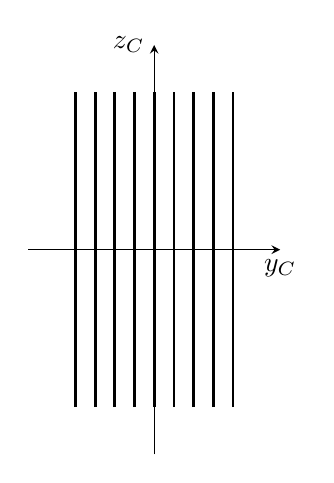
\begin{tikzpicture}
			\def\axisl{2};
			\def\zd{1};
			\draw[-stealth] (-0.8*\axisl,0) -- (0.8*\axisl,0) node[below]{$y_C$};
			\draw[-stealth] (0,-1.3*\axisl) -- (0,1.3*\axisl) node[left]{$z_C$};
			
			\draw[line width=0.35mm] (-1,-\axisl/\zd) -- (-1,\axisl/\zd);
			\draw[line width=0.35mm] (-0.75,-\axisl/\zd) -- (-0.75,\axisl/\zd);
			\draw[line width=0.35mm] (-0.5,-\axisl/\zd) -- (-0.5,\axisl/\zd);
			\draw[line width=0.35mm] (-0.25,-\axisl/\zd) -- (-0.25,\axisl/\zd);
			
			\draw[line width=0.35mm] (0,-\axisl/\zd) -- (0,\axisl/\zd);
			
			\draw[line width=0.35mm] (0.25,-\axisl/\zd) -- (0.25,\axisl/\zd);
			\draw[line width=0.35mm] (0.5,-\axisl/\zd) -- (0.5,\axisl/\zd);
			\draw[line width=0.35mm] (0.75,-\axisl/\zd) -- (0.75,\axisl/\zd);
			\draw[line width=0.35mm] (1,-\axisl/\zd) -- (1,\axisl/\zd);
			\end{tikzpicture}
			\small{Raggio uniforme}
		\end{subfigure}
		\hfill
		\begin{subfigure}{.3\textwidth}
			\centering
			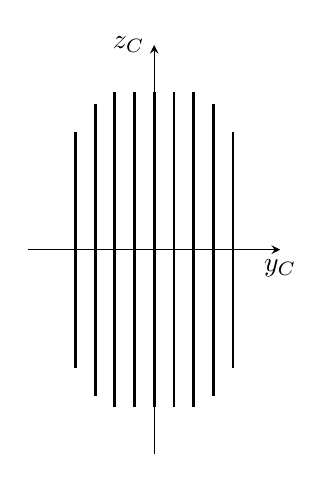
\begin{tikzpicture}
			\def\axisl{2};
			\def\zd{1};
			\draw[-stealth] (-0.8*\axisl,0) -- (0.8*\axisl,0) node[below]{$y_C$};
			\draw[-stealth] (0,-1.3*\axisl) -- (0,1.3*\axisl) node[left]{$z_C$};
			
			\draw[line width=0.35mm] (-1,-\axisl/\zd+0.5) -- (-1,\axisl/\zd-0.5);
			\draw[line width=0.35mm] (-0.75,-\axisl/\zd+0.5-0.5*1.41/2) -- (-0.75,\axisl/\zd-0.5+0.5*1.41/2);
			\draw[line width=0.35mm] (-0.5,-\axisl/\zd) -- (-0.5,\axisl/\zd);
			\draw[line width=0.35mm] (-0.25,-\axisl/\zd) -- (-0.25,\axisl/\zd);
			
			\draw[line width=0.35mm] (0,-\axisl/\zd) -- (0,\axisl/\zd);
			
			\draw[line width=0.35mm] (0.25,-\axisl/\zd) -- (0.25,\axisl/\zd);
			\draw[line width=0.35mm] (0.5,-\axisl/\zd) -- (0.5,\axisl/\zd);
			\draw[line width=0.35mm] (0.75,-\axisl/\zd+0.5-0.5*1.41/2) -- (0.75,\axisl/\zd-0.5+0.5*1.41/2);
			\draw[line width=0.35mm] (1,-\axisl/\zd+0.5) -- (1,\axisl/\zd-0.5);
			\end{tikzpicture}
			\small{Spalla raccordata}
		\end{subfigure}
		\hfill
		\begin{subfigure}{.3\textwidth}
			\centering
			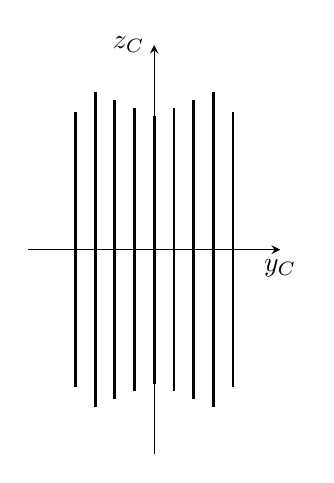
\begin{tikzpicture}
			\def\axisl{2};
			\def\zd{1};
			\draw[-stealth] (-0.8*\axisl,0) -- (0.8*\axisl,0) node[below]{$y_C$};
			\draw[-stealth] (0,-1.3*\axisl) -- (0,1.3*\axisl) node[left]{$z_C$};
			
			\draw[line width=0.35mm] (-1,-\axisl/\zd+0.25) -- (-1,\axisl/\zd-0.25);
			\draw[line width=0.35mm] (-0.75,-\axisl/\zd) -- (-0.75,\axisl/\zd);
			\draw[line width=0.35mm] (-0.5,-\axisl/\zd+0.1) -- (-0.5,\axisl/\zd-0.1);
			\draw[line width=0.35mm] (-0.25,-\axisl/\zd+0.2) -- (-0.25,\axisl/\zd-0.2);
			
			\draw[line width=0.35mm] (0,-\axisl/\zd+0.3) -- (0,\axisl/\zd-0.3);
			
			\draw[line width=0.35mm] (0.25,-\axisl/\zd+0.2) -- (0.25,\axisl/\zd-0.2);
			\draw[line width=0.35mm] (0.5,-\axisl/\zd+0.1) -- (0.5,\axisl/\zd-0.1);
			\draw[line width=0.35mm] (0.75,-\axisl/\zd) -- (0.75,\axisl/\zd);
			\draw[line width=0.35mm] (1,-\axisl/\zd+0.25) -- (1,\axisl/\zd-0.25);
			\end{tikzpicture}
			\small{Profilo personalizzato}
		\end{subfigure}
		\hfill
	\end{figure}
\end{frame}

\begin{frame}[fragile]
	\Large{Istanziamento dello pneumatico}:
	\normalsize
\begin{pseudoc}
TireGround::Tire* TireSD = new TireGround::MagicFormula(
SectionWidth, // [m]
AspectRatio,  // [%]
RimDiameter,  // [in]
SwitchNumber  // Max triangles in the shadow
);
\end{pseudoc}
\begin{pseudoc}
TireGround::Tire* TireMD = new TireGround::MultiDisk(
SectionWidth, // [m]
AspectRatio,  // [%]
RimDiameter,  // [in]
RadiusVec,    // Disks radius vector [m]
PointsNumber, // Sampling points for each disk
SwitchNumber  // Max triangles in the shadow
);
\end{pseudoc}
\end{frame}

\begin{frame}
	\Large{Intersezione con la mesh}:
	\normalsize
	\begin{enumerate}
		\item Modello di contatto di Rill
	\end{enumerate}
\end{frame}

\begin{frame}
	\Large{Contatto per rappresentazione a singolo disco}:
	\normalsize
	\begin{enumerate}
		\item Modello di contatto di Rill
	\end{enumerate}
\end{frame}

\begin{frame}
	\begin{enumerate}\addtocounter{enumi}{1}
		\item Modello di contatto ponderato in base all'area d'intersezione
	\end{enumerate}
\end{frame}

\begin{frame}
	\Large{Contatto per rappresentazione a più dischi}:
	\normalsize
	\begin{enumerate}
		\item Modello di contatto ponderato in base all'area d'intersezione
	\end{enumerate}
\end{frame}

\begin{frame}
	\begin{enumerate}\addtocounter{enumi}{1}
		\item Modello di contatto tramite campionamento
	\end{enumerate}
\end{frame}

\begin{frame}
	\Large {La libreria}:
	
\end{frame}

\begin{frame}
	\Large {Prestazioni}:

\end{frame}

\begin{frame}
	\Large {Conclusioni}:
	
\end{frame}

\end{document}